\documentclass{article}

\usepackage{hyperref}
\usepackage{amsmath}
\usepackage{amsfonts}
\usepackage{amssymb}
\usepackage{listings}
\usepackage{graphicx}
\usepackage{color}
\usepackage{float}
\definecolor{mauve}{RGB}{204,153,255}
\definecolor{mylilas}{RGB}{200,162,200}
\definecolor{pageno}{gray}{0.30}

\title{IS Physics Problem Set 1} \date{27-08-2015} \author{Hrishi Olickel}

\begin{document}
 \pagenumbering{gobble}
 \maketitle
 \newpage
 
\graphicspath{ {/} }
\lstdefinestyle{MATLAB}{ % 
    %basicstyle=\color{red},
    language = Matlab,
    breaklines=true,%
    morekeywords={matlab2tikz},
    frame=single,
    keywordstyle=\color{blue},%
    morekeywords=[2]{1}, keywordstyle=[2]{\color{black}},
    identifierstyle=\color{black},%
    stringstyle=\color{mylilas},
    commentstyle=\color{green},%
    showstringspaces=false,%without this there will be a symbol in the places where there is a space
    numbers=left,%
    numberstyle={\tiny \color{black}},% size of the numbers
    numbersep=9pt, % this defines how far the numbers are from the text
    emph=[1]{for,end,break},emphstyle=[1]\color{red}, %some words to emphasise
    %emph=[2]{word1,word2}, emphstyle=[2]{style},    
} 

\lstset{style=MATLAB}

 \section{Part a}

Let us consider the system at the point where we diverge using the small angle approximation:

\begin{equation}
\frac{d^2\theta}{dt^2}+\frac{g}{l} sin\,\theta = 0
\end{equation}
It is at this point that we would assume $sin \theta \approx \theta$. But we can still make the assumption that the function for theta would resemble a sine curve, and that it relates to its amplitude, $\theta _0$. Therefore,

\begin{equation}
\theta = A\,sin(\theta_0 t)
\end{equation}
\begin{equation}
\frac{d\theta}{dt} = A\,cos(\theta_0 t)
\end{equation}
\begin{equation}
\frac{d^2\theta}{dt^2} = - A\,sin(\theta_0 t)
\end{equation}

Substituting (4) and (2) into (1), we get

\begin{equation}
 A\,sin(\theta_0\,t)+\frac{g}{l} sin(A\,sin(\theta_0\,t)) = 0
\end{equation}
\begin{equation}
\therefore  A\,sin(\theta_0\,t)= -\frac{g}{l} sin (A\,sin(\theta_0\,t))
\end{equation}

This is a considerably difficult equation to solve, so let us see what the relationship between the two variable terms here are. Let us graph sin(x) and sin(sin(x)) on the same axes:

\begin{figure}[H]
\caption{Red - sin(x), Blue - sin(sin(x))}
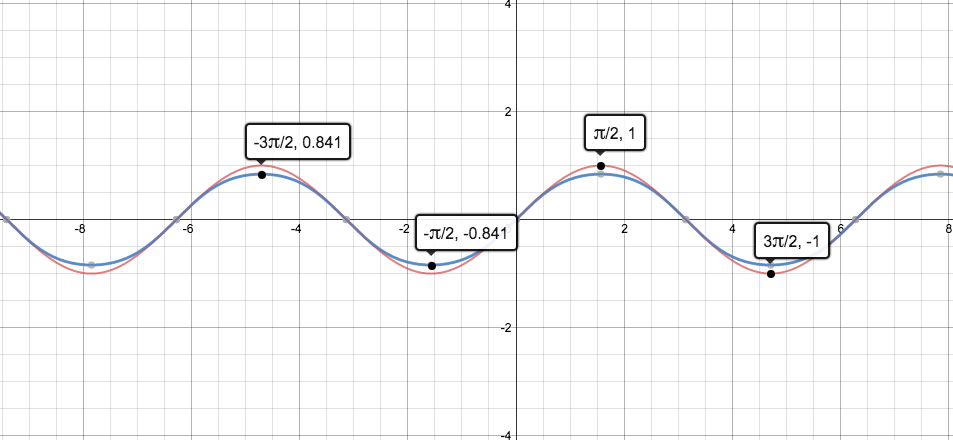
\includegraphics[width=\textwidth]{ExternalGraph}
\end{figure}

Solving this equation means arriving at a solution for the constants $\theta_0$ and $A$ that would make these two graphs equal, in a sense. But looking at the graph we can see that a simple solution wouldn't be possible, and that an approximation is the best option. Here we rest, hoping for the advent of computers.
 
\section{Part b}

Without modifying the original code for oscillator.m, we can easily modify the calculation functions to solve for a simple pendulum:

Firstly, calcForce is modified to use the equation of restoring force for a simple pendulum:
\begin{lstlisting}
function F = calcForce(m, x)
    % Take current x coordinate and return force acting on mass
    F = -m*9.81*sin(x);
end
\end{lstlisting}

Next, calcAccel is modified to include the length parameter for the pendulum, for conversion from angular velocity to velocity:
\begin{lstlisting}
function aNow = calcAccel(F, mass, length)
    % Take force and mass and return acceleration based Newtons second law    
    aNow = F/(mass*length);
end
\end{lstlisting}

The other elements are left the same as they are, with the understanding that variables of x now hold values of theta. A damping constant \emph{dampC} is added to adjust damping, and damping is introduced in the for loop show below (only relevant code is shown for the sake of brevity\footnote{The full code for oscillator.m can be found at \url{http://pastebin.com/zumTEJWj}.}:

\begin{lstlisting}
    %%% Initial conditions %%%
    initX = pi/4;
    initV = 5;
    mass = 1;
    length = 1;
    dampC = 0;

    vNow = initV;
    xNow = initX;
    timeNow = 0;

    %%% Time handling %%%
    totalTime = 10*2*pi; %Total time to simulate
    N = 10000; % Number of simulation steps (more = more accuracy)
    delT = totalTime/N;  %Time for each time step

    %%% Arrays to store time points and associated x values %%%
    tSteps = [];
    xSteps = [];
    vSteps = [];
    dispSteps = [];
    pxSteps = [];
    pySteps = [];
    
    %%% main "for" loop - do N steps if simulation %%%%
    for step = 1:1:N, 
        fNow = calcForce(mass, xNow);   % calculate force at point x
        
        damping = dampC*vNow; %calculate damping
        fNow  = fNow - damping; %adjust force accordingly
        aNow = calcAccel(fNow,mass,length);   % calculate acceleration at point x
        
        xNow = xNow + calcDeltaX(vNow,aNow,delT);   % update x (location)
        vNow = vNow + calcDeltaV(aNow,delT);   % update velocity
        timeNow = timeNow+delT;    % update time
        
        tSteps = [tSteps, timeNow];  % store current time for plotting
        xSteps = [xSteps, xNow];  % store current location for plotting
        vSteps = [vSteps, vNow];
        dispNow = length*xNow;
        dispSteps = [dispSteps, dispNow];
        pxSteps = [pxSteps, length * sin(xNow)];
        pySteps = [pySteps, -(length * cos(xNow))];
      
    end
\end{lstlisting}

Without damping, the following plot is produced:

\begin{figure}[H]
\caption{Time Simulated: $2\times\pi$, mass=1, length=1}
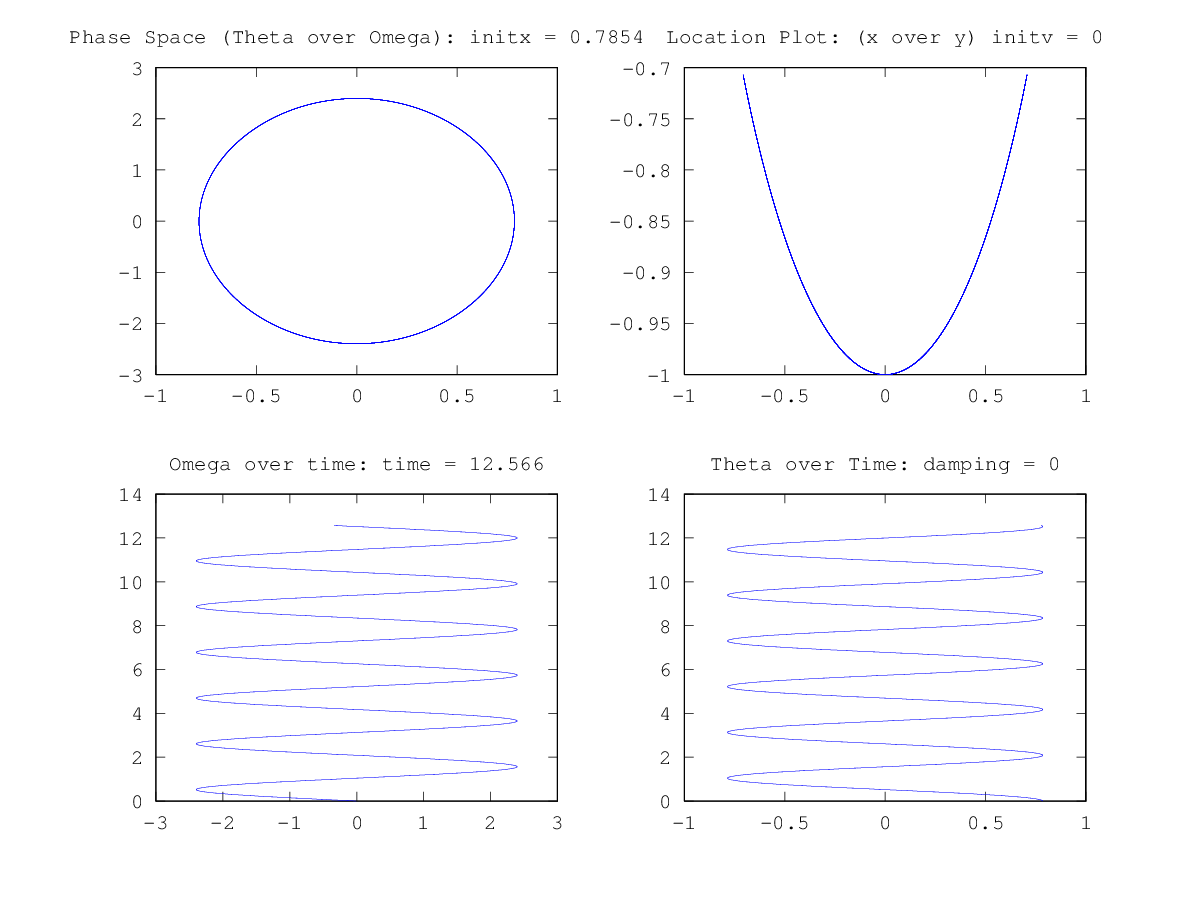
\includegraphics[width=\textwidth]{plot1}
\end{figure}

For very high initial velocity, the pendulum goes over the top (the location plot is now a complete circle): 
\begin{figure}[H]
\caption{Time Simulated: $2\time\pi$, mass=1, length=1}
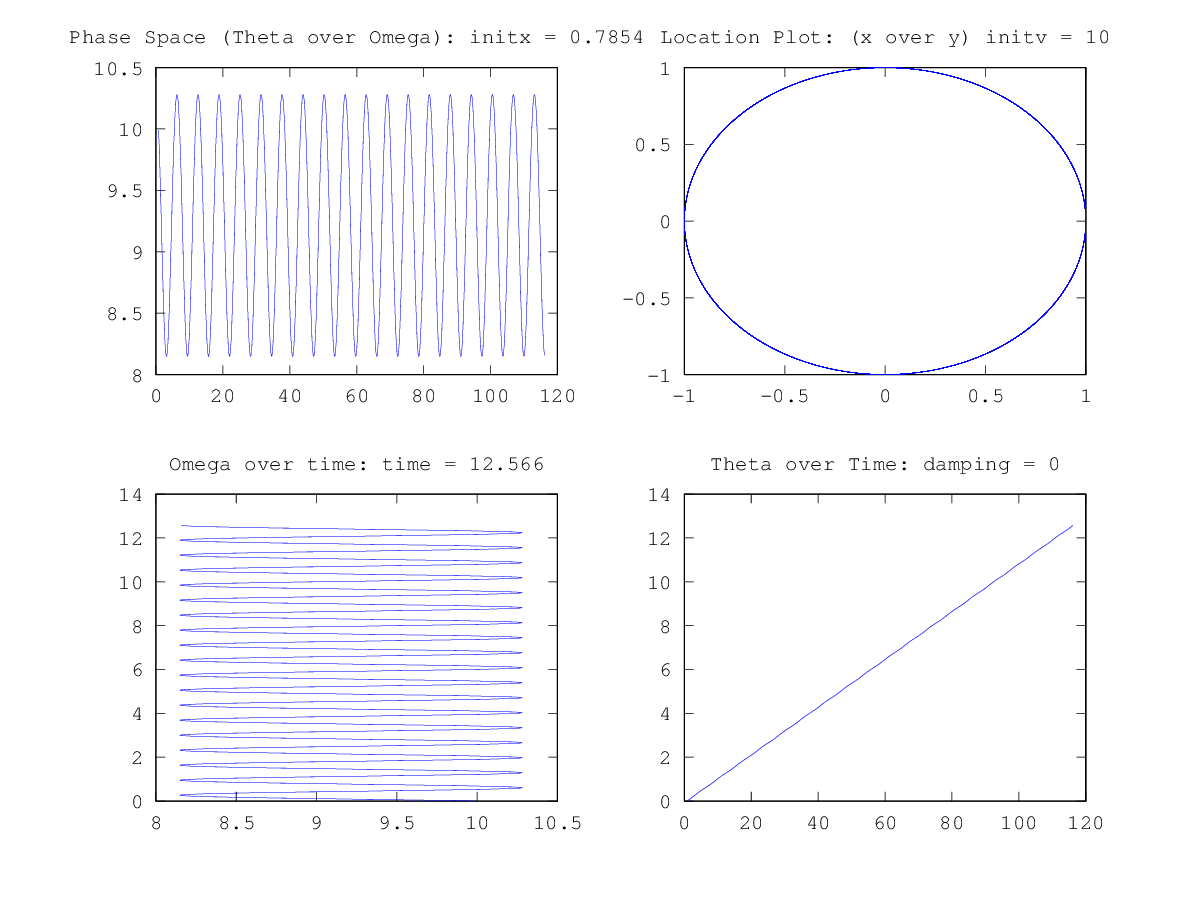
\includegraphics[width=\textwidth]{plot2}
\end{figure}

We can also see that the movement does not settle into a single phase space. Now, with damping:

\begin{figure}[H]
\caption{Time Simulated: $2\times\pi$, mass=1, length=1}
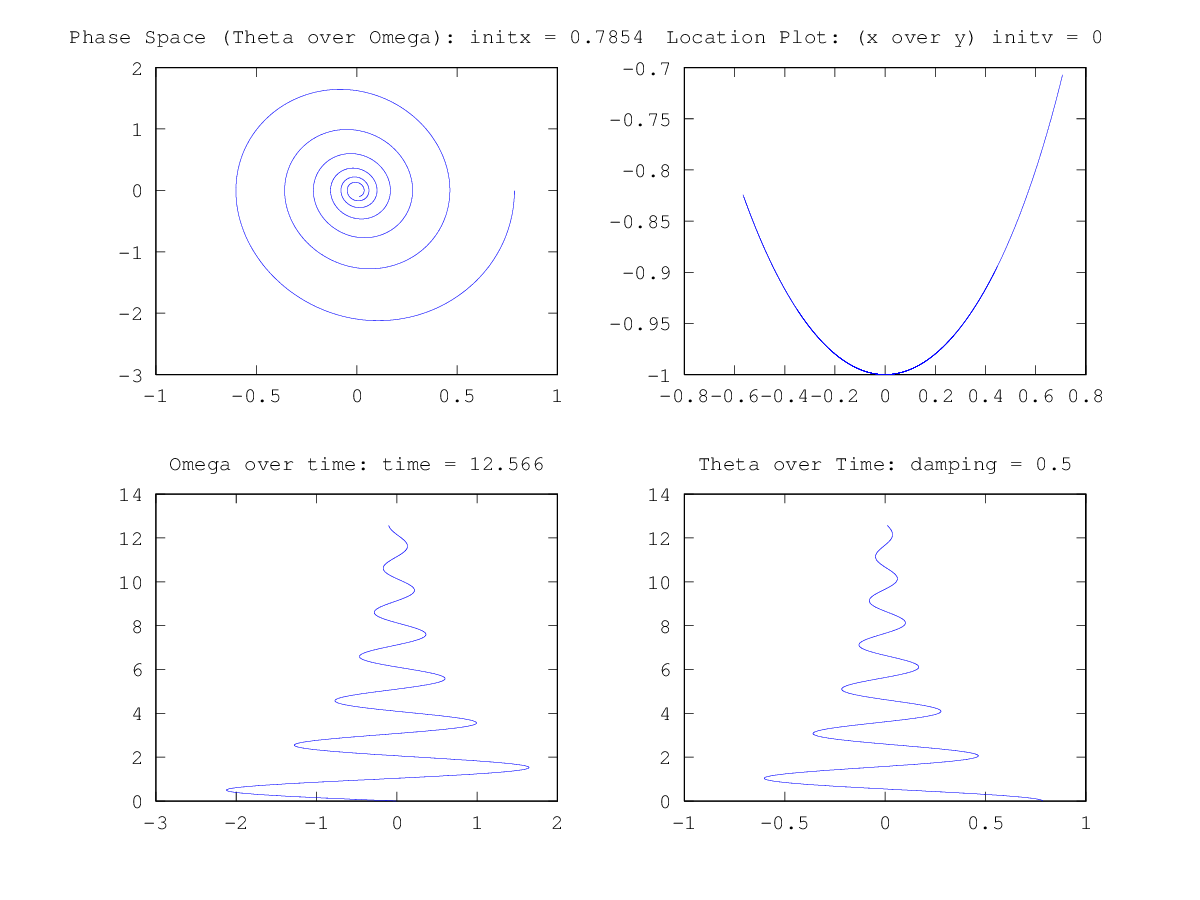
\includegraphics[width=\textwidth]{plot3}
\end{figure}

We can see the phase space spiral into the center.
What if we were to increase the initial velocity and position so it goes over the top? 

\begin{figure}[H]
\caption{Time Simulated: $2\times\pi$, mass=1, length=1}
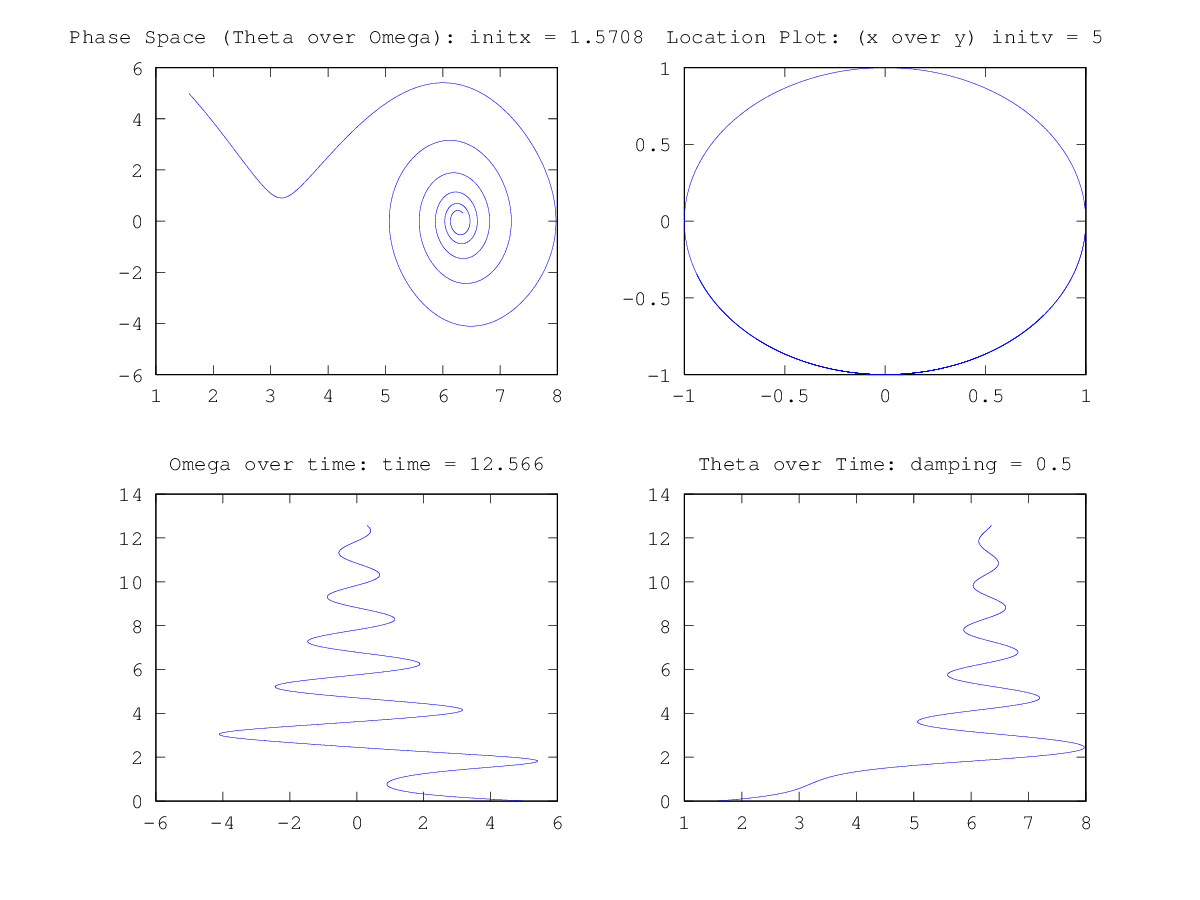
\includegraphics[width=\textwidth]{plot4}
\end{figure}

We can see that the pendulum goes over the top once, but settles into the next stable state where damping eventually leads it to rest.

An even higher velocity shows the pendulum moving to different possible loops in phase space before eventually not having enough energy and begin oscillating.

This is a good example of where the small angle approximation would not work very well. The error term is compounded with each rotation instead of cancelling out when $\theta$ is zero. After a few rotations the estimates are very far removed from observational or numerical results.

\begin{figure}[H]
\caption{Time Simulated: $2\times\pi$, mass=1, length=1}
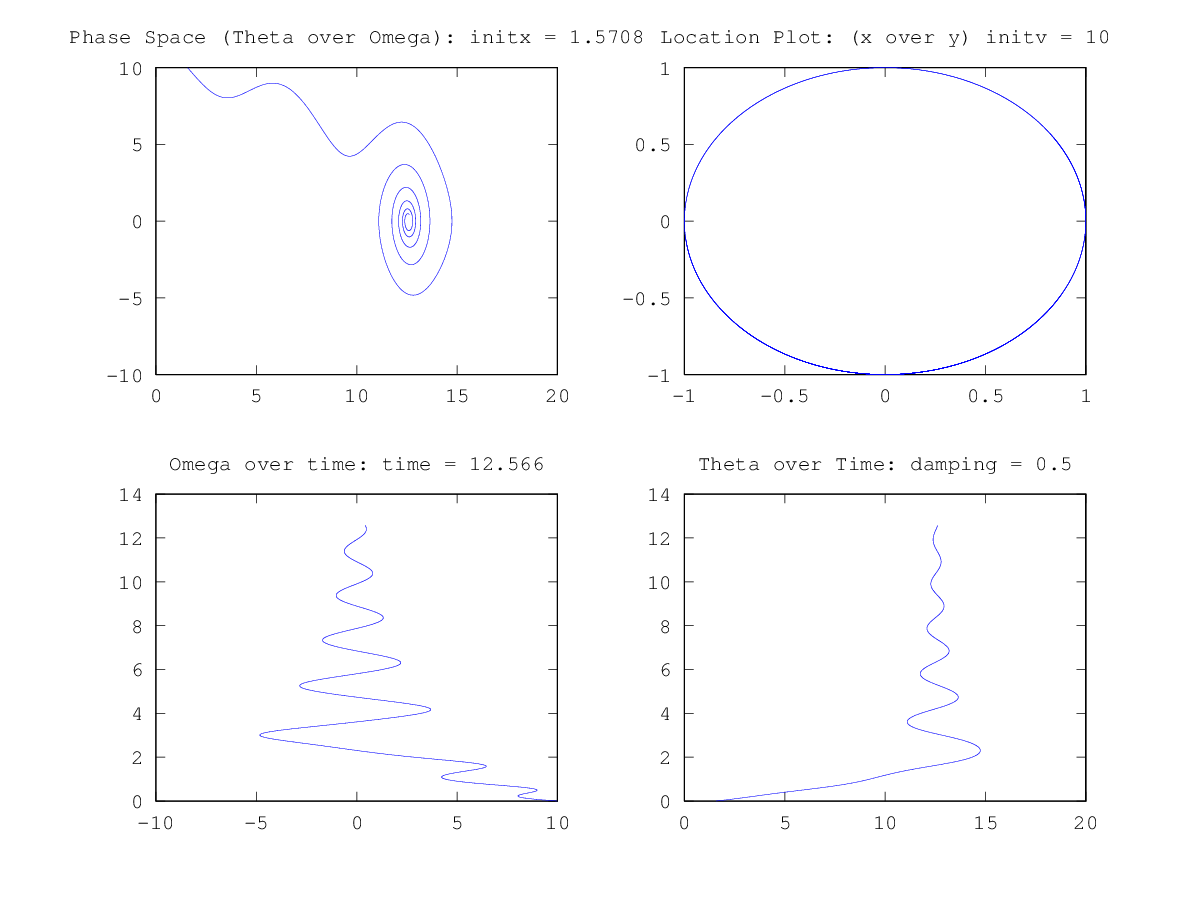
\includegraphics[width=\textwidth]{plot5}
\end{figure}

\newpage
\section{Part C}
The input function xdot\footnote{The complete code for the vector field plotter (plotGraphs.m) can be found at \url{http://pastebin.com/f01GbgMw}} was created for plotting the vector field: 
\begin{lstlisting}
function xdot = f(x,t)
      dampC = 0.5;
      % x(1) is theta, x(2) is omega
      length = 1;
      mass = 1;
      f = -mass*9.81*sin(x(1))-(dampC*x(2));
      xdot(2) = f/(mass*length);
      xdot(1) = x(2);
    endfunction
\end{lstlisting}

When solved using lose and plotted using the vector field, a pendulum without damping can be seen:

\begin{figure}[H]
\caption{Time Simulated: $20\times\pi$, mass=1, length=1, initX=$\pi / 4$, initV=0, damping=0}
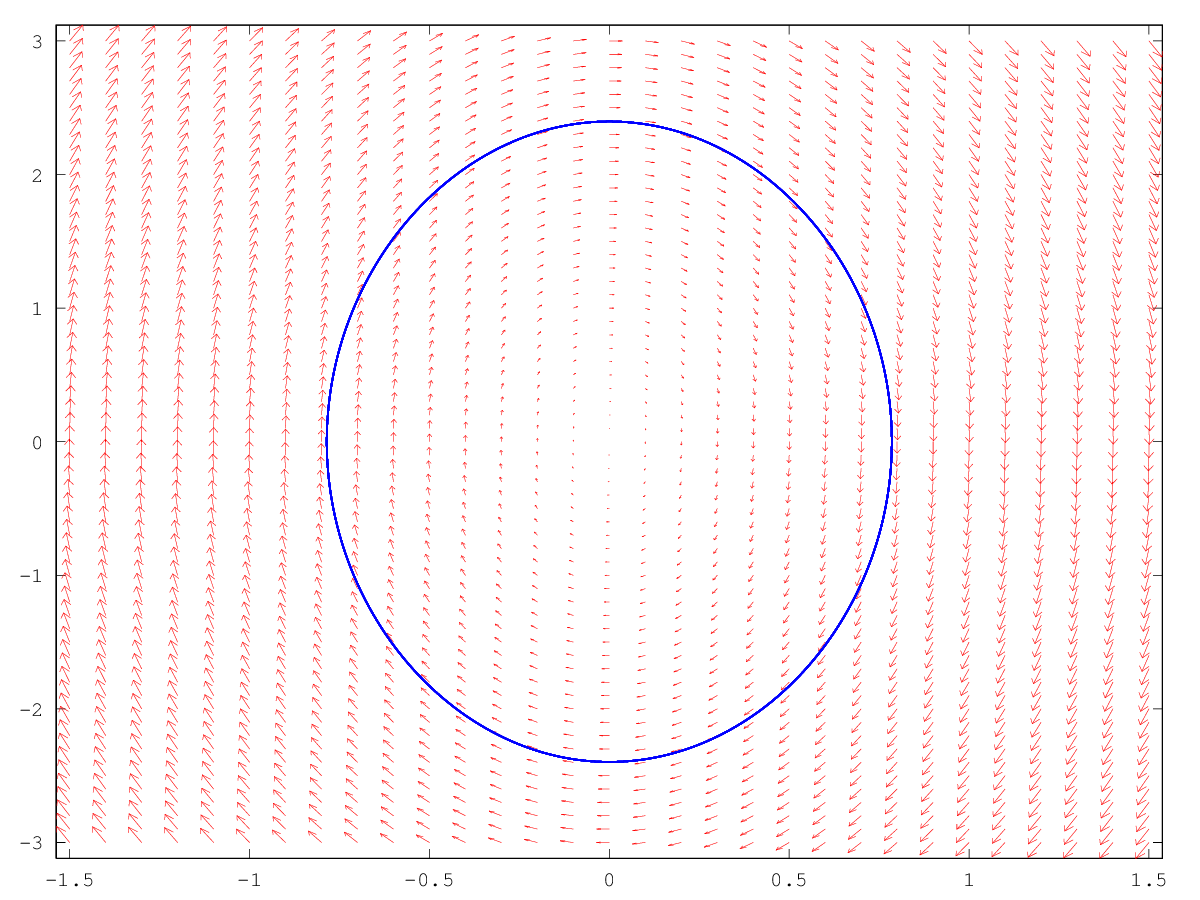
\includegraphics[width=\textwidth]{plot7}
\end{figure}

With damping:
\begin{figure}[H]
\caption{Time Simulated: $20\times\pi$, mass=1, length=1, initX=$\pi / 4$, initV=0, damping=0.5}
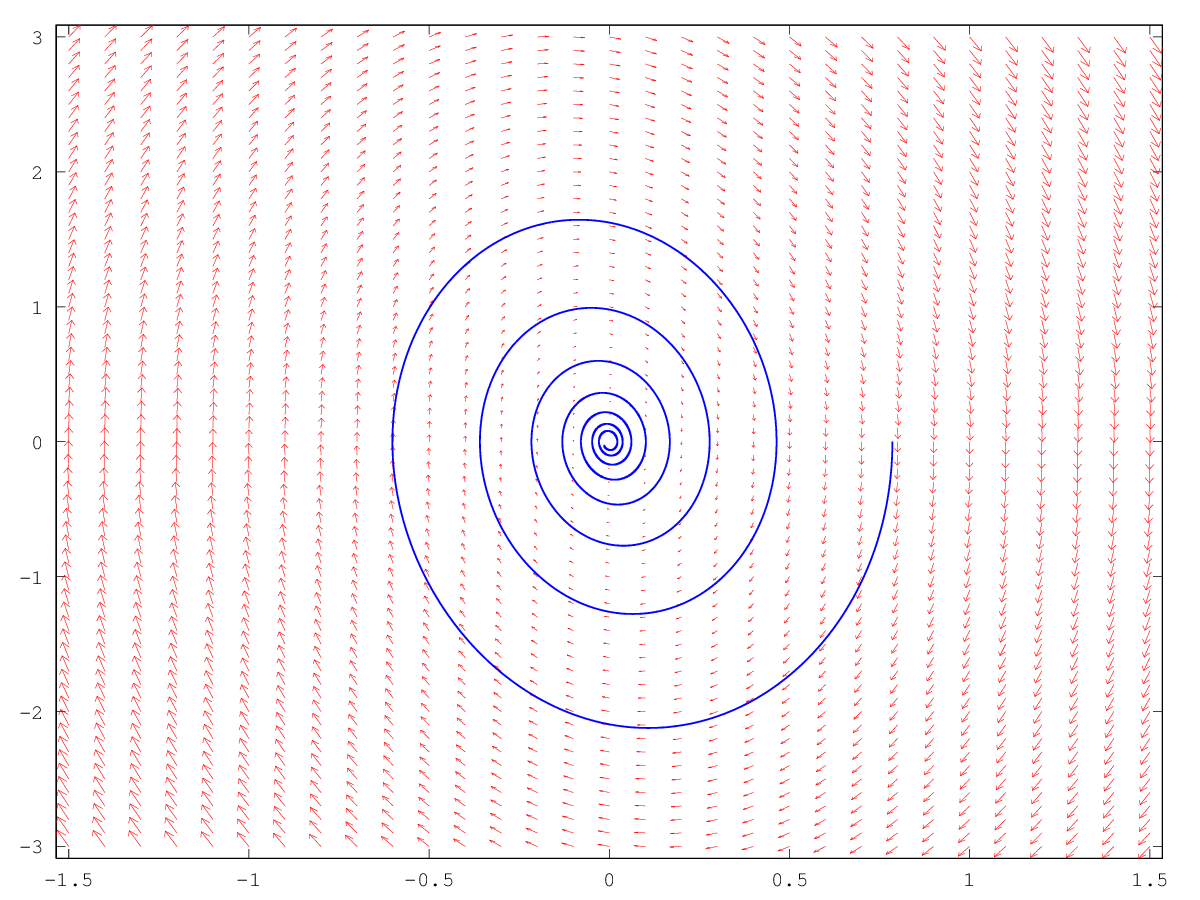
\includegraphics[width=\textwidth]{plot8}
\end{figure}

Careful observation points out how damping affects the vector field. An increase in damping reduces the the length of vectors as we move away from the origin. This decrease in strength causes the trajectory to spiral inward.

\newpage
\section{Part D}
The ode solver was used to plot the trajectory on top of the vector field in part C. The code is using the same function - xdot - used in part C, and the ODE solution can be obtained using a single line of code:

\begin{lstlisting}
x = lsode("f", [pi/4;0], (t = linspace(0,15,20000)'));
\end{lstlisting}
\newline
It is notable that the ODE solution is obtained much faster than Part B and especially Part C due to the adaptive time stepping of the solver. Part C is extremely intensive in terms of computing power required, as the nested loops scale in complexity by $O(n^2)$. In our case, the solver returns the value of 2, indicating an absence of roots, but that the entire timespace was solvable.

\section{Part E}
We have already looked at open and close trajectories for the pendulum, but let us plot a few trajectories along with the vector fields. The following is a closed trajectory, where the pendulum oscillates back and forth without damping:

\begin{figure}[H]
\caption{Time Simulated: $20\times\pi$, mass=1, length=1, initX=$\pi / 4$, initV=0, damping=0}
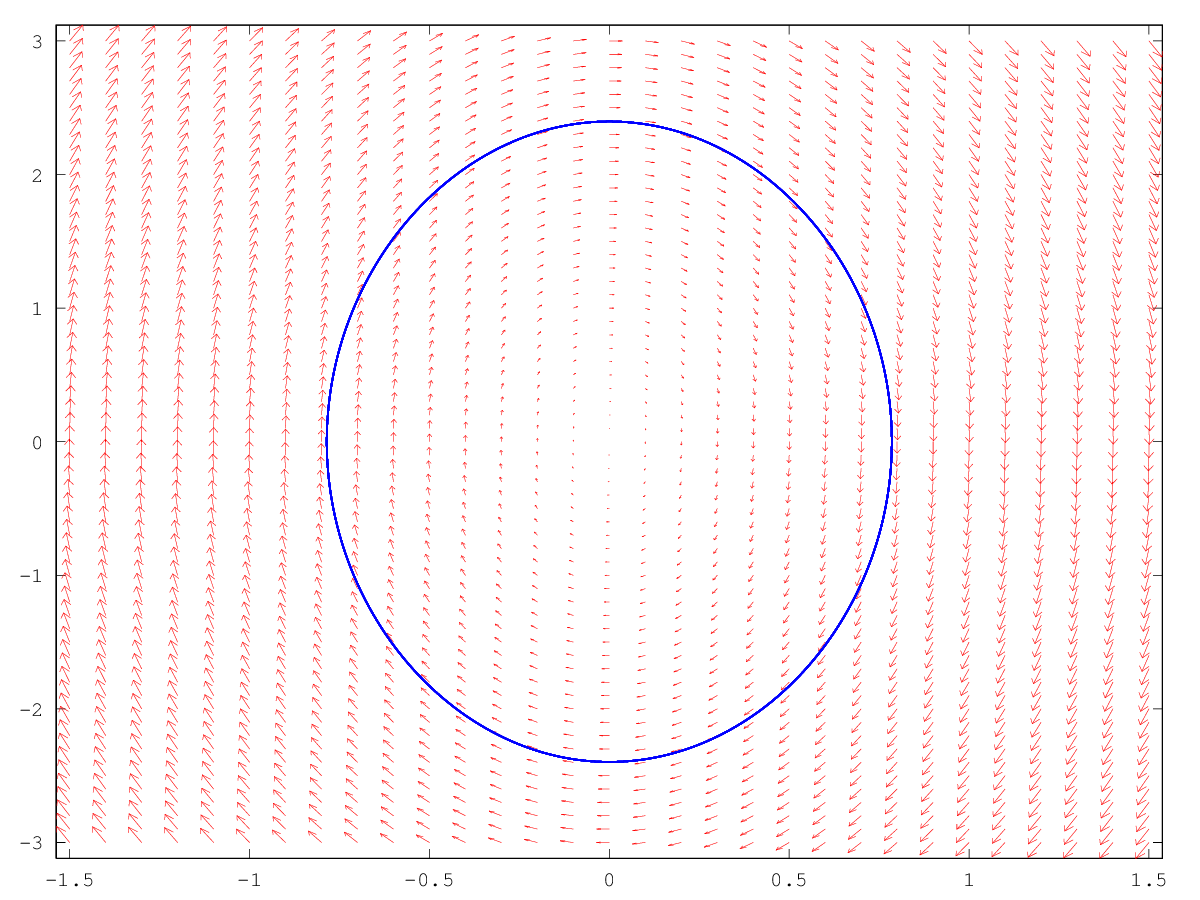
\includegraphics[width=\textwidth]{plot9}
\end{figure}

Without any damping, if we increase initial angle and velocity so that the pendulum were to go over the top, it would simply keep rotating forever:

\begin{figure}[H]
\caption{Time Simulated: $20\times\pi$, mass=1, length=1, initX=$\pi / 2$, initV=5, damping=0}
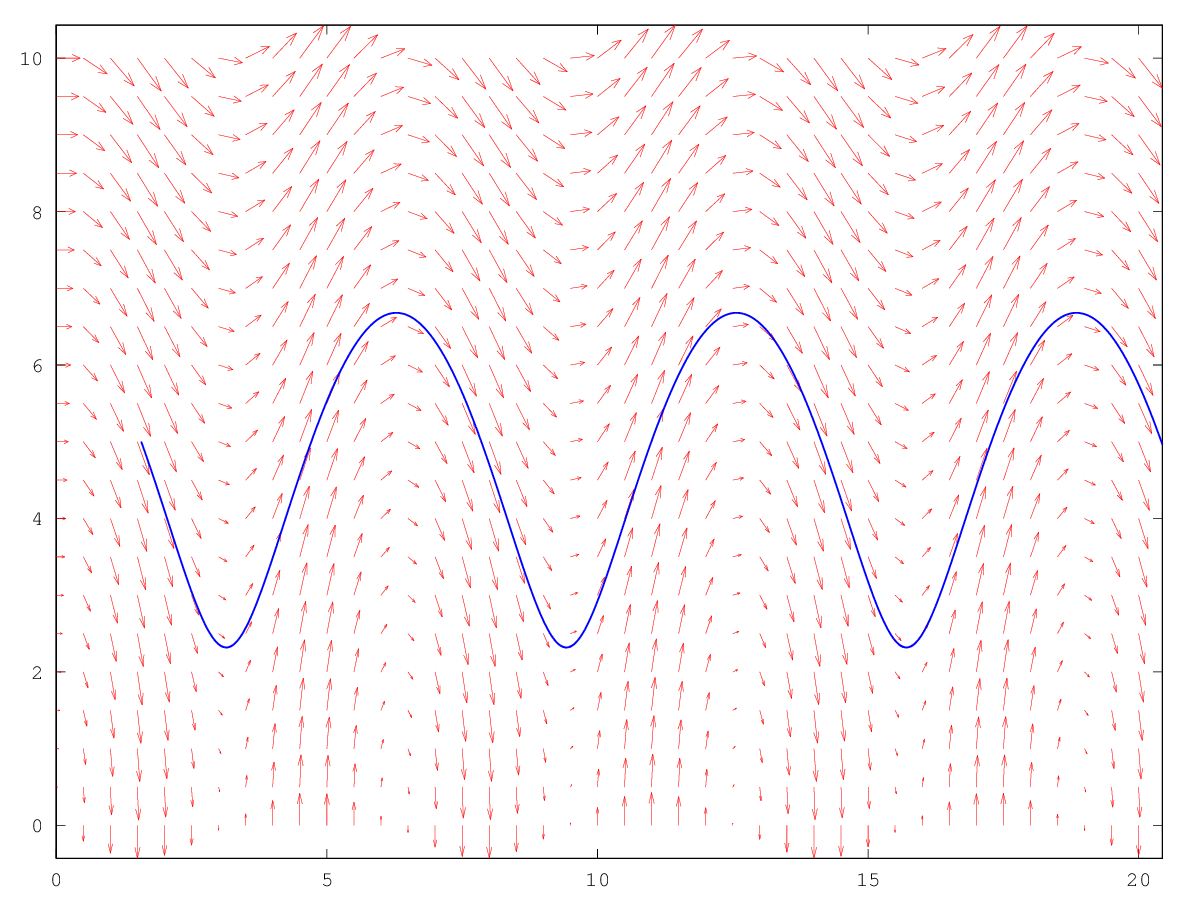
\includegraphics[width=\textwidth]{plot10}
\end{figure}

If we add damping, we can see similar behaviour as before, where the pendulum rotates until it doesn't have energy to keep rotating. It then returns to oscillation and eventually rest.

\begin{figure}[H]
\caption{Time Simulated: $20\times\pi$, mass=1, length=1, initX=$\pi / 4$, initV=0}
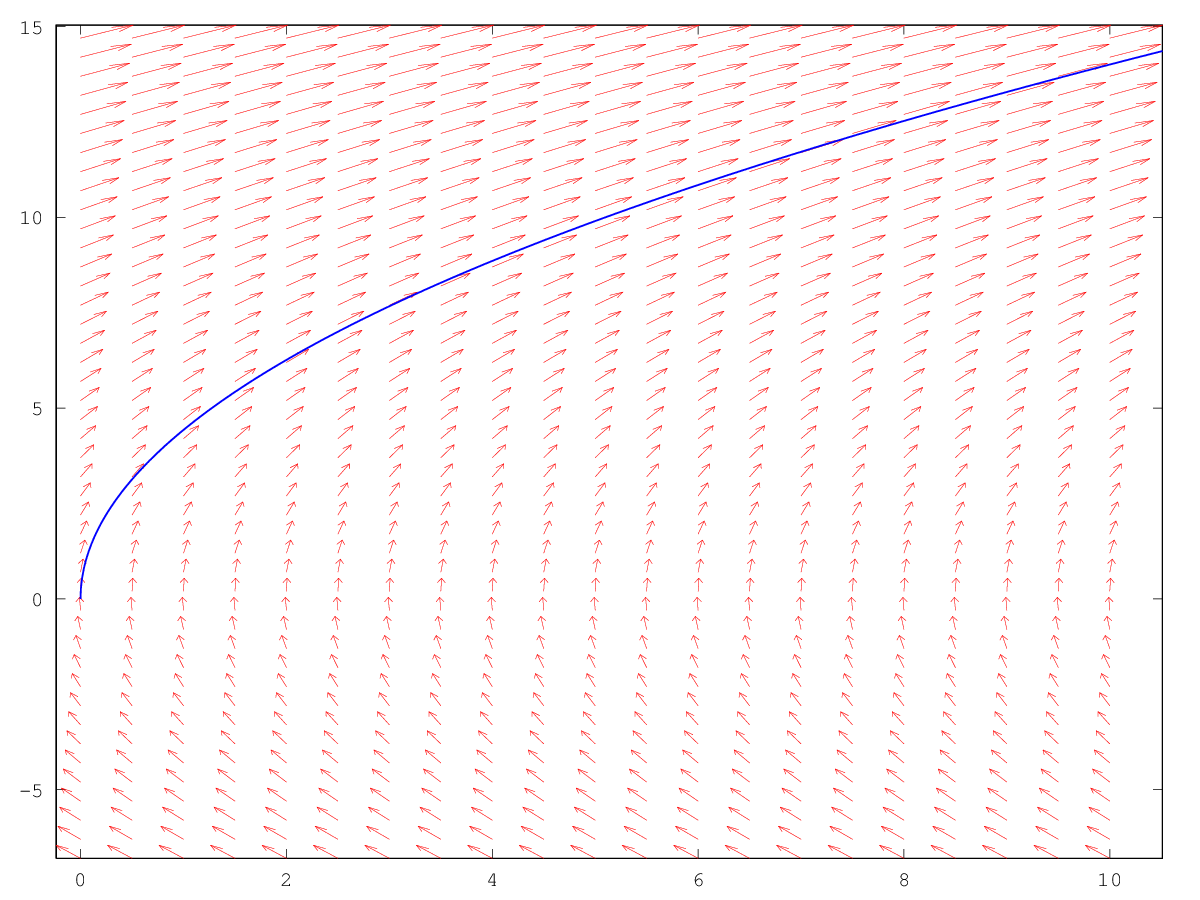
\includegraphics[width=\textwidth]{plot11}
\end{figure}

We can see that damping is removing energy from the pendulum with each rotation. With each rotation, it moves lower and lower in phase space until it crosses the separatrix, at which point it enters a new configuration, one that spirals toward the center. If damping were removed at this point, it would oscillate forever.

In this case, the separatrix is the exact angular momentum above which the pendulum rotates, and below which the pendulum oscillates. There is also a third condition, where the pendulum has just enough angular momentum to reach the top, and enters an unstable equilibrium, resting at the very top of it's motion. This, unfortunately for me, has been impossible to simulate (although I suspect an analytical solution can be found).

\end{document}
 